% Section 3 - Real-Time Applications
% Alessandro Tenaglia <alessandro.tenaglia@uniroma2.it>
% May 6, 2022

% ### Real Time Applications ###
\section{Real-Time Applications}
\graphicspath{{figs/section3/}}

% --- Real-Time Applications ---
\begin{frame}{Real-Time Applications}
	\begin{itemize}
		\item MARTe2 offers a generic base application, see \textbg{MARTeApp.cpp};
		\item Real-Time Applications are built from the base one through a \textbg{Configuration Files} (.cfg);
		\item The \textbg{Configuration Files} defines the algorithms to be executed (\textbg{GAMs}) and the hardware or software involved (\textbg{Data Sources}).
	\end{itemize}
\end{frame}

% --- Configuration file: RT App ---
\begin{frame}[fragile]{Configuration file: RT App}
	\begin{columns}\column{.9\textwidth}
		\begin{lstlisting}[style=small, language=cfg]
$RTApp = {
  Class = RealTimeApplication
  +Functions = { // GAMs
    Class = ReferenceContainer
    ...
  }
  +Data = { // Data Sources
    Class = ReferenceContainer
    ...
  }
  +States = { // RT States
    Class = ReferenceContainer
    ...
  }
  +Scheduler = { // Scheduler
    ...
  }
}\end{lstlisting}
	\end{columns}
\end{frame}

% --- GAMs ---
\begin{frame}{GAMs}
	\only<1,3>{
		\begin{block}{Generic Application Module}
			The \textbf{GAMs} are the components where user-algorithms are to be implemented.
		\end{block}
	}
	\only<2>{
		\begin{figure}
			\centering
			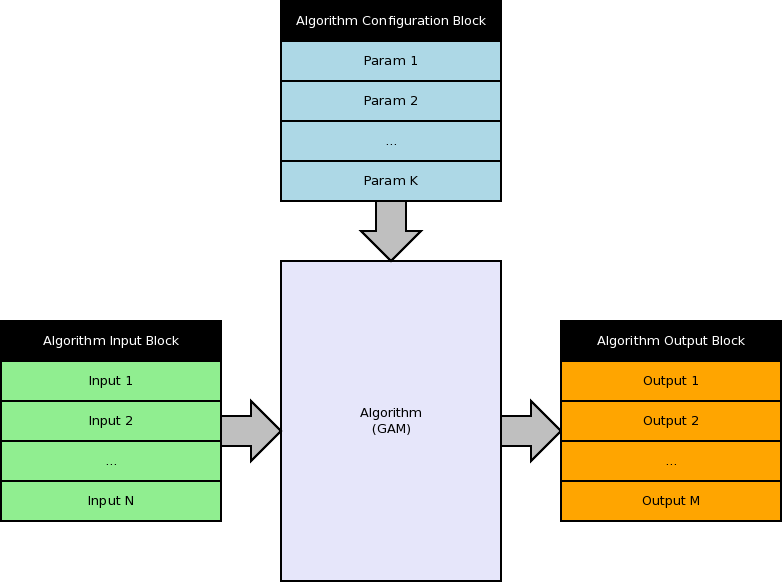
\includegraphics[scale=.33]{GAMs.png}
			\label{fig:gams}
			\caption{GAM}
		\end{figure}
	}
	\only<3>{
		\begin{alertblock}{Warning}
			No interface with operating system (e.g. reading from files/sockets)
		\end{alertblock}
	}
\end{frame}

\begin{frame}[fragile]{Configuration file: GAMs}
	\begin{columns}\column{.8\textwidth}
		\begin{lstlisting}[style=small, language=cfg]
+GAM1 = {
  Class = ExampleGAM
  InputSignals = {
    Input1 = {
      DataSource = DDB1
      Type = uint32
    }
  }
  OutputSignals = {
    Output1 = {
      DataSource = DDB1
      Type = uint32
    }
  }
  Parameters = {
	  Param1 = (uint32) 1000
  }
}\end{lstlisting}
	\end{columns}
\end{frame}

% --- DataSoruces ---
\begin{frame}{Data Sources \& Brokers}
	\begin{block}{Data Sources}
		The \textbf{Data Sources} are the components that provide a interface for the interchange of input and output signals with the memory and the hardware.
	\end{block}
	\begin{block}{Brokers}
		The \textbf{Brokers} are the components that provide the interface between the GAMs memory and the DataSource data.
	\end{block}
	\begin{figure}
		\centering
		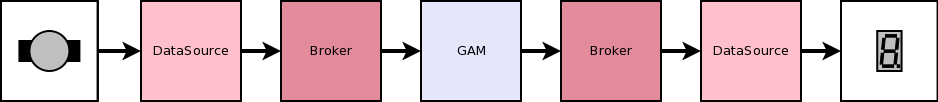
\includegraphics[scale=.35]{DataSources.png}
		\label{fig:datasources}
		\caption{Data Sources \& Brokers}
	\end{figure}
\end{frame}

\begin{frame}[fragile]{Configuration file: Data Sources}
	\begin{columns}\column{.8\textwidth}
		\begin{lstlisting}[style=small, language=cfg]
+Data = { // Data Sources
  Class = ReferenceContainer
  +DDB1 = {
    Class = GAMDataSource
  }
  +Timer = {
    Class = LinuxTimer
    SleepNature = Default
    Signals = {
      Counter = {
	    Type = uint32
	  }
      Time = {
        Type = uint32
      }
    }
	...
  }
}\end{lstlisting}
	\end{columns}
\end{frame}

% --- States ---
\begin{frame}{States}
	\begin{itemize}
		\item \textbg{GAMs} are grouped in real-time \textbg{threads} which are executed in the context of specific \textbg{states}.
		\item A Real-Time application shall be in one (\textbf{and only one}) state at a given time.
	\end{itemize}
\end{frame}
\begin{frame}[fragile]{Configuration file: States}
	\begin{columns}\column{.8\textwidth}
		\begin{lstlisting}[style=small, language=cfg]
+States = { // RT States
  Class = ReferenceContainer
  +State1 = {
    Class = RealTimeState
    +Threads = {
      Class = ReferenceContainer
      +Thread1 = {
        Class = RealTimeThread
        CPUs = 0x8
        Functions = {GAMTimer}
      }
      ...
    }
  }
  ...
}\end{lstlisting}
	\end{columns}
\end{frame}

% --- Scheduler ---
\begin{frame}[fragile]{Configuration file: Scheduler}
	\begin{itemize}
		\item A \textbg{real-time scheduler} handles thread execution;
	\end{itemize}
	\vspace{1cm}
	\begin{columns}\column{.8\textwidth}
		\begin{lstlisting}[style=normal, language=cfg]
+Scheduler = { // Scheduler
  Class = GAMScheduler
  TimingDataSource = Timings
}\end{lstlisting}
	\end{columns}
\end{frame}

% --- RTApp  ---
\begin{frame}{Example: Real-Time Application}
	\begin{figure}
		\centering
		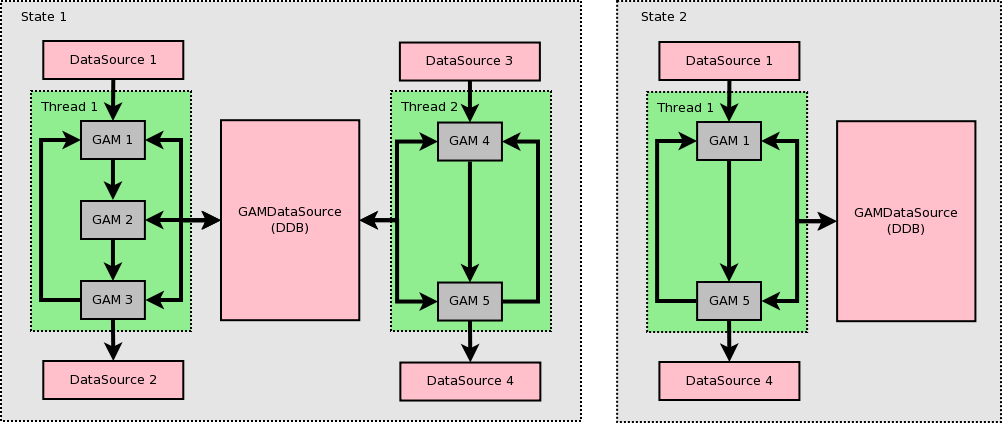
\includegraphics[width=\textwidth]{RTApp.png}
		\label{fig:rtapp_example}
		\caption{Example of a multi-state and multi-threaded real-time application}
	\end{figure}
\end{frame}
